\section{EXPERIMENTS}\label{sec:expe}
The main focus of the experiments section is to demonstrate the trip scoring. Primarily to demonstrate the possibility to score similar routes differently, based on the calculated metrics stored in the system. Therefore, a policy is created using parameters and variables found reasonable by the authors. An insurance company would have to decide on these parameters for policies offered to customers. The chosen parameters and values can be seen in the tables \ref{tab:roadtypevalues}, \ref{tab:crittimevalues}, \ref{tab:speedingvalues}, \ref{tab:accelerationvalues}, \ref{tab:basevalues}, and \ref{tab:polyvalues}.

\begin{table}
    \centering
    \begin{tabular}{ll}
    \textbf{Roadtype} & \textbf{Weight} \\ \hline
    Motorway          & 1               \\
    Trunk             & 1               \\
    Primary           & 1               \\
    Secondary         & 1.05            \\
    Tertiary          & 1.1             \\
    Unclassified      & 1.1             \\
    Residential       & 1.2             \\
    Service           & 1.2             \\ \hline
    \end{tabular}
    \caption{Roadtypes with weights}
    \label{tab:roadtypevalues}
\end{table}

\begin{table}
    \centering
    \begin{tabular}{llll}
    \textbf{Active days} & \textbf{Start} & \textbf{End} & \textbf{Weight} \\ \hline
    Monday - Friday      & 07:00:00       & 09:00:00     & 1.2             \\
    Monday - Friday      & 15:00:00       & 17:00:00     & 1.15            \\
    Saturday - Sunday    & 09:00:00       & 13:00:00     & 1.025           \\
    Saturday - Sunday    & 20:00:00       & 23:59:59     & 1.15            \\
    Saturday - Sunday    & 00:00:00       & 00:04:00     & 1.4             \\ \hline
    \end{tabular}
    \caption{Critical time intervals with weights}
    \label{tab:crittimevalues}
\end{table}

\begin{table}
    \centering
    \begin{tabular}{ll}
    \textbf{Interval (\%)}   & \textbf{Weight} \\ \hline
    {[}0, 10{[}        & 1.3                   \\
    {[}10, 20{[}       & 1.4                   \\
    {[}20, 30{[}       & 1.5                   \\
    {[}30, 40{[}       & 1.6                   \\
    {[}40, 50{[}       & 1.7                   \\
    {[}50, 60{[}       & 1.8                   \\
    {[}60, 70{[}       & 1.9                   \\
    {[}70, $\infty${]} & 2                     \\ \hline
    \end{tabular}
    \caption{Speeding intervals with weights}
    \label{tab:speedingvalues}
\end{table}

\begin{table}
    \centering
    \begin{tabular}{ll}
    \textbf{Interval (m/s)} & \textbf{Weight} \\ \hline
    {[}0, 3{[}              & 1               \\
    {[}3, 5{[}              & 1               \\
    {[}5, 7{[}              & 1.075           \\
    {[}7, 8{[}              & 1.1             \\
    {[}8, 9{[}              & 1.2             \\
    {[}9, 10{[}             & 1.4             \\
    {[}10, 11{[}            & 1.6             \\
    {[}11, $\infty${]}      & 1.9             \\ \hline
    \end{tabular}
    \caption{Acceleration, brake and jerk intervals with weights}
    \label{tab:accelerationvalues}
\end{table}

\begin{table}
    \centering
    \begin{tabular}{ll}
    \textbf{Action} & \textbf{Base weight} \\ \hline
    Acceleration    & 50                   \\
    Brake           & 75                   \\
    Jerk            & 62.5                 \\ \hline
    \end{tabular}
    \caption{Base weights for accelerations, brakes and jerks}
    \label{tab:basevalues}
\end{table}

\begin{table}
    \centering
    \begin{tabular}{ll}
    \textbf{Parameter} & \textbf{Weight} \\ \hline
    A                  & 1.02            \\
    B                  & 1.05            \\
    C                  & 0               \\
    Polynomial degree  & 1.08            \\ \hline
    \end{tabular}
    \caption{Weights for all polynomial functions}
    \label{tab:polyvalues}
\end{table}

To test this policy, and thereby the developed scoring system, trips were handpicked from the INFATI dataset\cite{art:INFATI}. This was done on the following criteria:

\begin{itemize}
  \item Trips should follow similar routes
  \item Trips should be similar in distance
  \item Trips should display different driving styles
\end{itemize}

From these criteria, two different test cases were picked. The trips included in these cases are visualized in figures \ref{fig:shorttrips} and \ref{fig:longtrips} with two and three trips respectively. The first being two short-distance trips, and second being three long-distance trips.

\subsection{Experiment 1: Short trips} \label{subsec:expe1}
The trips chosen for experiment 1 are visualized in Figure \ref{fig:shorttrips} and represents two $\sim$8.1km trips with a similar route. They are driven back and forth with the same car, on the same day. The route driven is simple and has very few turns. The trips are visualized using a green and red color.

\begin{figure}[tb]
    \centering
    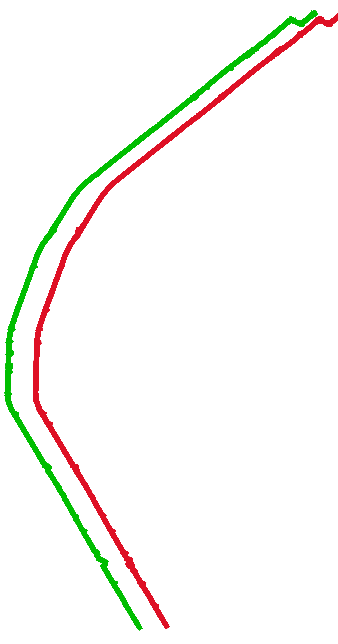
\includegraphics[width=40mm]{Pictures/ShortTrips.png}
    \caption{Green and red route for experiment 1}
    \label{fig:shorttrips}
\end{figure}

For naive usage-based-insurance, the car owners would be accountable for just the distance driven. Thus, the trips would cost approximately the same. With the authors developed advanced usage-based-insurance approach, it is demonstrated why this assessment of the cost is faulty.

Looking at the metrics from this test case (See Table  \ref{tab:shorttrips}), accelerations, brakes and jerks are very similar, both in count and distribution across intervals. The green trip has slightly higher counts, but the distributions reveal no clear winner across the categories. While the trips are driven on the same route, these metric-similarities are not guaranteed, but can possibly be attributed to it being the same driver driving both trips. The metric where the two trips really differentiate themselves from each other is Speeding. In spite of the similarities in the driving pattern, the car sped over three times more on green trip, compared to red trip. 3.24 kilometers of speeding on an 8.08 kilometer trip is significant, and should cost more than the 1.02 kilometers of speeding on red trip.

The calculated tripscores for experiment 1 can be seen in table \ref{tab:shorttripscores}. The base score for both trips is identical to the distance driven denoted in meters. A slight difference can be seen on road-types, in spite of the routes being near identical. This can be attributed to very subtle deviations like the timing of each GPS point when roadtypes change or the success of the map-matching algorithm used. The biggest difference is as expected: Due to the excessive speeding the green trip is charged an additional 1564.05 meters, compared to red trip. Accelerations, brakes and jerks are also judged to be slightly worse, although the difference is more subtle. In the end green trip pays for over 12 kilometers, despite driving only $\sim$8.1 kilometers. Red trip is substantially less with 10.3 kilometers, but still some way from the possible 8478.08 meters that a careful driver might achieve, given that the influence of roadtypes are considered uncontrollable.

\begin{table}
    \centering
    \begin{tabular}{lll}
    \textbf{Score type} & \textbf{Green trip} & \textbf{Red trip} \\ \hline
    Base                & 8076,23             & 8070,52           \\
    RoadType            & 355,35              & 407,56            \\
    Critical time       & 0                   & 0                 \\
    Speeding            & 2282,91             & 718,86            \\
    Acceleration        & 239,44              & 216,54            \\
    Brake               & 939,53              & 753,05            \\
    Jerk                & 213,27              & 158,06            \\ \hline
    \textbf{Total}      & \textbf{12106,72}   & \textbf{10324,60} \\ \hline
    \end{tabular}
    \caption{Trip score distribution for test case 1}
    \label{tab:shorttripscores}
\end{table}

\subsection{Experiment 2: Long trips} \label{subsec:expe2}
The trips chosen for the experiment 2 can be seen in figure \ref{fig:longtrips}. These are longer and more complex trips between $\sim$31.7km and $\sim$32.0km in distance. These trips have more turns and are driven on a mix of roadtypes. The red and green are driven by the same driver, whereas the purple is from a different car.

\begin{figure}[tb]
    \centering
    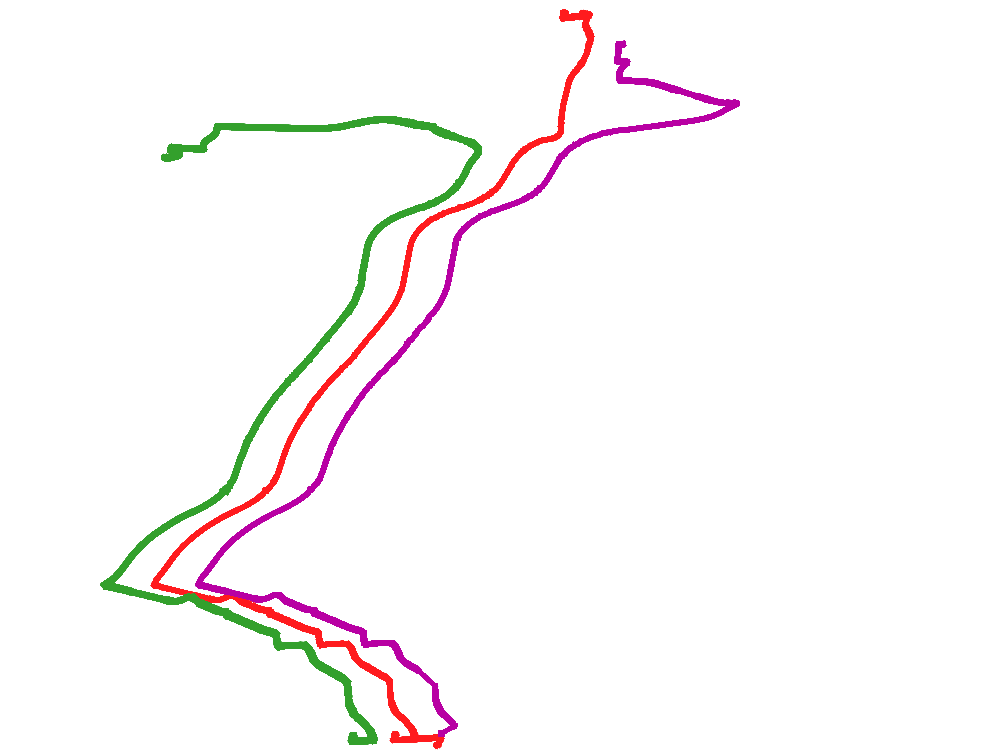
\includegraphics[width=80mm]{Pictures/LongTrips.png}
    \caption{Green, red and purple route for experiment 2}
    \label{fig:longtrips}
\end{figure}

This test case is a three-way comparison and the routes are not exactly the same, although they share a majority of the same segments, as seen in figure \ref{fig:longtrips}. Looking at Table \ref{tab:longtrips}, the differences in metrics are very clear. Green trip is driven extremely well compared to the other two; low counts on accelerations, brakes and jerks, and intervals exclusively in the low end, and almost no speeding. Note that the total counts on this trip are about as low as the trips in test case 1 (See table \ref{tab:shorttrips}), despite being approximately 4 times as long.
Looking at red trip for comparison, we have a vast increase in all counts; More accelerations, brakes and jerks, and worse distribution of the intervals. A total of 31.76 kilometers driven, 13.06 kilometers of these were driven above the speed limit, mostly in the interval of 20-30\% above the speed limit.

Note that despite of the massive differences in metrics, both of these trips were driven by the same car. Whether this indicates the driver being in a rush on green trip, or a different driver is difficult to predict with single examples - but the differences are clear.

The purple trip is as mentioned driven by a different car. Looking at acceleration, brake and jerk counts along with the amount of speeding in table \ref{tab:longtrips}, the trip is clearly positioned between the other two trips. The matching intervals provides an extended view on these counts, indicating that this driver consistently makes rapid changes in speed. Both acceleration, brake and jerk intervals reached higher values than 11 on several occasions. The worst offender is the jerks distribution - 56\% of the jerks is positioned in the worst interval 11$m/s^3$ or above that. This is a striking contrast to the green and red trip, in which the worst case for this interval is 8\% on braking.

The aggregated scores seen in \ref{tab:longtripscores} are as expected given the driving patterns. Red trip is very expensive due to the excessive speeding, and the sheer amount of changes in speed. Green trip comes very close to the best possible score of 32764.82(base $+$ roadtype) for a route of 32043.83 meters. The extra cost from driving style adds up to only 825.57 meters(all metrics). Purple trip is charged extra for driving on a Tuesday morning where heavier traffic is expected. In spite of red trip having higher counts of accelerations brakes and jerks in total amounts, purple trip cost more on these points combined. This is due to the distributions which were significantly worse for the purple trip, meaning each delinquency has been significantly more severe.

\begin{table}
    \centering
    \begin{tabular}{llll}
    \textbf{Score type} & \textbf{Green trip} & \textbf{Red trip} & \textbf{Purple trip}\\ \hline
    Base                & 32043,83            & 31763,97          & 31660,97            \\
    RoadType            & 720,99              & 873,51            & 696,54              \\
    Critical time       & 0                   & 0                 & 237,46              \\
    Speeding            & 8,96                & 12291,53          & 2544,64             \\
    Acceleration        & 115,16              & 431,74            & 914,66              \\
    Brake               & 317,33              & 1996,90           & 1778,41             \\
    Jerk                & 384,12              & 998,09            & 2857,83             \\ \hline
    \textbf{Total}      & \textbf{33590,39}   & \textbf{48355,73} & \textbf{40690,52}   \\ \hline
    \end{tabular}
    \caption{Trip score distribution for test case 2}
    \label{tab:longtripscores}
\end{table}

\begin{table*}
    \centering
    \begin{tabular}{>{\bfseries}l|ll|}
    Figure color             & Green               & Red                 \\
    Car ID                   & 16                  & 16                  \\
    Weekday                  & Thursday            & Thursday            \\
    Start                    & 18:35:59            & 19:02:22            \\
    End                      & 18:44:15            & 19:11:24            \\
    Distance (km)            & 8.08                & 8.07                \\
    Distance sped (km)       & 3.24                & 1.02                \\
    Accelerations ($>$5m/s)  & 23                  & 21                  \\
    Brakes ($>$5m/s)         & 40                  & 38                  \\
    Jerks ($>$5m/s)          & 15                  & 14                  \\
    Roadtype intervals       & 0 0 0 88 0 0 0 0    & 0 0 0 93 0 0 2 0    \\
    Speeding intervals       & 56 41 2 2 0 0 0 0   & 62 28 5 5 0 0 0 0   \\
    Acceleration intervals   & 0 0 87 0 4 9 0 0    & 0 0 67 10 24 0 0 0  \\
    Brake intervals          & 0 0 48 20 18 10 5 0 & 0 0 50 24 16 11 0 0 \\
    Jerk intervals           & 0 0 60 20 13 7 0 0  & 0 0 71 14 14 0 0 0  \\
    \end{tabular}
    \caption{Trip data for test case 1}
    \label{tab:shorttrips}
\end{table*}

\begin{table*}
    \centering
    \begin{tabular}{>{\bfseries}l|lll|}
    Figure color            & Green                & Red                 & Purple             \\
    Car ID                  & 10                   & 10                  & 14                 \\
    Weekday                 & Friday               & Sunday              & Tuesday            \\
    Start                   & 22:42:35             & 18:56:50            & 08:56:15           \\
    End                     & 23:11:42             & 19:23:45            & 09:29:19           \\
    Distance (km)           & 32.04                & 31.76               & 31.67              \\
    Distance sped (km)      & 0.02                 & 13.06               & 3.63               \\
    Accelerations ($>$5m/s) & 16                   & 49                  & 34                 \\
    Brakes ($>$5m/s)        & 29                   & 71                  & 55                 \\
    Jerks ($>$5m/s)         & 21                   & 56                  & 41                 \\
    Roadtype intervals      & 49 10 00 27 5  0 2 0 & 54 0 0 29 7 0 3 0   & 58 0 0 30 3 0 2 0  \\
    Speeding intervals      & 100 0 0 0 0 0 0 0    & 02 29 62 06 0 0 0 0 & 78 5 4 13 0 0 0 0  \\
    Acceleration intervals  & 0 0 94 6 0 0 0 0     & 0 0 84 6 8 2 0 0    & 0 0 68 3 6 0 3 21  \\
    Brake intervals         & 0 0 90 10 0 0 0 0    & 0 0 61 13 10 6 3 8  & 0 0 62 11 5 9 0 13 \\
    Jerk intervals          & 0 0 57 24 10 5 0 5   & 0 0 64 16 7 7 4 2   & 0 0 32 5 5 2 0 56  \\
    \end{tabular}
    \caption{Trip data for test case 2}
    \label{tab:longtrips}
\end{table*}